\clearpage
\section{Effect typing}
\label{System:Effects}

% --------------------
\subsection{Effects and interference}
\label{System:Effects:interference}
When the evaluation of an expression performs read or write actions on mutable data, the compiler must ensure that these actions occur in the correct order, else the meaning of the program will change. We have seen how region variables are used to reason about the \emph{mutability} of data, and we now discuss how to reason about the actions. Following Talpin and Jouvelot \cite{talpin:discipline} we use \emph{effect typing} to annotate function types with a description of the actions each function performs. 

For example, the $\iinc$ function reads its argument, computes the successor, and writes the new value back to its argument. Adding this information to the type gives us:

\code{
 	$\iinc$ 
	& $::$		& $\forall r_1. \ \iInt \ r_1 \lfuna{\iRead \ r_1 \ \lor \ \iWrite \ r_1} ()$ \\
	& $\rhd$	& $\iMutable \ r_1$
}

The effect annotation on the function arrow tells us which regions in the store will be accessed when it evaluates. When the effect term becomes large this syntax is hard to read. For this reason we usually introduce an \emph{effect variable}, and add a constraint to the type that contains the original effect term:

\code{
	$\iinc$ 
	& $::$		& \mc{2}{$\forall r_1. \ \iInt \ r_1 \funa{e_1} ()$} \\
	& $\rhd$	& $e_1 = \iRead \ r_1 \lor \iWrite \ r_1$ \\
	& ,	 	& \mc{2}{$\iMutable \ r_1$}

}

Effect variables are identified as $e_n$ in this text, and as variables preceded by an exclamation mark\footnote{a mnemonic for: ``something's happening!"} \texttt{!en} in the concrete syntax. The exclamation mark is used as both a namespace qualifier and as the symbol for effect kinds. In the concrete syntax, effect constructors such as \texttt{!Read} and \texttt{!Write} are also preceded by this namespace qualifier. Akin to value type constructors, the effect constructors have specific kinds. Both $\iRead$ and $\iWrite$ take a region and produce an effect, so we have:

\code{
	$\iRead$	& $:: \% \to \ !$ \\
	$\iWrite$	& $:: \% \to \ !$
}

Treating the function constructor as a general type constructor, we can read the infix application $a \funa{e} b$ as shorthand for the prefix application $(\to) \ a \ b \ e$. This will help when presenting the typing rules of the core language, as we can use general type application to build function types instead of requiring a rule specific to functions.

Single, \emph{atomic effects} such as $\iRead \ r_1$ and $\iWrite \ r_1$ are gathered together with the join operator $\lor$. Effects form a lattice ordered by set inclusion on atomic effects. We use $\sigma_1 \sqsubseteq \sigma_2$ to mean effect $\sigma_1$ is no greater than effect $\sigma_2$, for example:

\code{
	$\iRead \ r_1 \tle  \iRead \ r_1 \lor \iWrite \ r_1$
}

The $\lor$ operator corresponds to set union. We use $\bot$ (bottom) to represent the effect of an expression which performs no visible actions, and a function arrow with no annotation is taken to have this effect. Conversely, we use $\top$ (top) to represent the effect of an expression which could perform all possible actions. This top element is useful because we can erase any effect term in our program by replacing it with $\top$, without loss of safety. We can also use $\top$ when the true effect of an expression is unknown. As we desire a top element in our effect structure, we use a lattice to gather effects instead of using sets directly. We also find the lattice notation more convenient, as we can write $\sigma \lor \iRead \ r_1$ instead of $\sigma \cup \{ \iRead \ r_1 \}$, where $\sigma$ is an arbitrary effect. The original effect system of Gifford and Lucassen \cite{gifford:integrating} is also presented as a lattice, though they do not use an explicit top element.

The notion of effect is intimately related to the notion of \emph{interference} \cite{reynolds:interference}, which relates to how the evaluation of one expression may affect the outcome of another. For example, if one expression has the effect $\iRead \ r_1$ and another has $\iWrite \ r_1$, then they \emph{may} be accessing the same heap object. In this case our compiler must worry about the order in which these two expressions are evaluated, and in particular, it must preserve this order when performing optimisations. Importantly, the notion of interference is separate from the usual method of propagating information between expressions via data dependencies. For example:

\code{
	$y = \idouble \ \ x$ \\
	$z = \isucc \ \ y$ 
}

The evaluation of the first statement is most certainly going to affect the outcome of the second, but we don't count this as interference, because changing their order would violate the scoping rules of the language and prevent the program from being compiled.

On the other hand, if we had:

\code{
	$y = \isucc \ x$ \\
	$\iinc \ z$
}

These two statements may or may not interfere, depending on whether $x$, $y$ or $z$ are aliases for the same object.

When speaking of effects, we pronounce $\bot$ as ``pure'', because the evaluation of an expression with this effect can be safely reordered with respect to any other. We pronounce $\top$ as ``sync'' because an expression with this effect may interfere with all other impure expressions, so it must be synchronised with respect to them all.

% ------------------
\subsection{Effect information in types}
\label{System:Effect:information-in-types}

Here is the type of $\iupdateInt$, which overwrites the value of its first argument with the second:

\code{
	$\iupdateInt$ 
	& $::$		& $\forall r_1 \ r_2. \ \iInt \ r_1 \to \iInt \ r_2 \lfuna{e_1} ()$ \\
	& $\rhd$	& $e_1 = \iWrite \ r_1 \ \lor \ \iRead \ r_2$ \\
       	& ,		& $\iMutable \ r_1$ 

}

\clearpage{}
When typeset, effect variables are written above the function arrow. However, in the concrete syntax we combine them with the arrow:

\begin{small}
\begin{lstlisting}
   updateInt :: forall %r1 %r2
             .  Int %r1 -> Int %r2 -(!e1)> ()
             :- !e1 = !{ !Write %r1; !Read %r2 }
             ,  Mutable %r1 
\end{lstlisting}
\end{small}

The syntax \texttt{!\{ !e1; !e2; ... \}} is equivalent to \mbox{$e1 \lor e2 \lor ...$}

All functions that write to a particular region also require that region to be mutable. When we express type signatures, we can leave out mutability constraints so long as we include the appropriate write effect. 

On the other hand, the inclusion of a mutability constraint does not imply that a function is necessarily capable of writing to the associated region. The effect information in a type gives an \emph{upper bound} on the particular actions a function may perform at runtime. For example, the following type signature is valid, but some of the information contained does not correspond to an actual property of the function:

\code{
	$\ireturnFive$
	& $::$		& $\forall r_1 \ r_2. \ \iInt \ r_1 \lfuna{e_1} \iInt \ r_2$ \\
	& $,$		& $e_1 = \iWrite \ r_1$ \\
	& $\rhd$	& $\iMutable \ r_1$ 
\\[1ex]
 	\mc{3}{$\ireturnFive \ x \ = \ 5$}
}

This is an example of \emph{effect weakening}. It is always safe to treat a particular function (or expression) as having a larger effect than it necessarily does. With regard to interference, weakening the effect of an expression corresponds to synchronising its evaluation with other parts of the program, more than we would strictly need to.

Returning to the type of $\iupdateInt$, the effect term we use for $e_1$ could really be anything we like, as long as it includes $\iWrite \ r_1 \lor \iRead \ r_2$. Indeed, we could weaken its type by quantifying $e_1$ and making this fact explicit:

\code{
	$\iupdateInt$ 
	& $::$		& $\forall r_1 \ r_2 \ e_1. \ \iInt \ r_1 \to \iInt \ r_2 \lfuna{e_1} ()$ \\
	& $\rhd$	& $e_1 \sqsupseteq \ \iWrite \ r_1 \lor \iRead \ r_2$ \\
        & ,	 	& $\iMutable \ r_1$ 
}

Writing this another way, we could place the $e_1 \sqsupseteq \iWrite \ r_1 \lor \iRead \ r_2$ constraint directly on the quantifier:

\code{
	$\iupdateInt$
	& $::$		& $\forall r_1 \ r_2 \ \ (e_1 \sqsupseteq \iWrite \ r_1 \lor \iRead \ r_2)$ \\
	& $.$		& $\iInt \ r_1 \to \iInt \ r_2 \lfuna{e_1} ()$ \\
	& $\rhd$ 	& $\iMutable \ r_1$
}

This new constraint gives a lower bound on the effect with which $e_1$ can be instantiated as. We will return to the practical differences between the strong and weak forms of $\iupdateInt$ in \S\ref{System:Effects:constraint-strengthening}

Note that although atomic effects have a textual ordering when collected together with $\lor$, there is no corresponding information in the analysis. In the type of $\iupdateInt$, the effect term $\iWrite \ r_1$ appears before $\iRead \ r_1$ on the page, yet clearly the function must read the source argument before it writes to the destination. The $\lor$ operator is commutative so $\sigma_1 \lor \sigma_2$ is equivalent to $\sigma_2 \lor \sigma_1$. 
For comparison, in the behavior types of Nielson and Nielson \cite{nielson:from-cml-to-its-process-algebra, nielson:type-and-effect-systems}, the order of actions is preserved.


% ---------------------
\subsection{Effects and currying}
\label{System:Effects:currying}
In our examples, usually only the right-most function arrow will have an effect annotation, though this is not required in general. Our primitive $\iupdateInt$ function needs both arguments before it can proceed, hence both $\iRead \ r_2$ and $\iWrite \ r_1$ appear on the same arrow.

If we partially apply $\iupdateInt$ by supplying just the first argument, then the runtime system will build a thunk. This thunk holds a pointer to the object code for the ``real'' primitive update function, along with a pointer to the supplied argument. Building a thunk has no visible effect on the rest of the program, so this partial application is pure. Only when we apply the second and final argument will the runtime system be in a position to call the primitive function to carry out the update action.

In contrast, we could define a slightly different function that reads the source argument as soon as it is applied:
\medskip

\code{
	\mc{3}{$\ireadThenUpdateInt$} \\
	& $::$		& $\forall r_1 \ r_2 . \ \iInt \ r_1 \lfuna{e_1} \iInt \ r_2 \lfuna{e_2} ()$ \\
	& $\rhd$ 	& $e_1 = \iRead \ r_1$ \\
	& ,		& $e_2 = \iWrite \ r_2$ \\
	& ,		& $\iMutable \ r_2$
}

\code{
	\mc{3}{$\ireadThenUpdateInt \isrc$} \\
	$\ \ =$	& $\kdo$	& $\isrc' = \icopyInt \ \isrc$ \\
 	  	& 		& $(\lambda \idest \to \iupdateInt \ \idest \ \isrc')$ \\
}

\qq where 

\code{
	\mc{3}{$copyInt$} \\
	& $::$		& $\forall r_1 \ r_2 . \ \iInt \ r_1 \lfuna{e_1} \iInt \ r_2$ \\
	& $\rhd$	& $e_1 = \iRead \ r_1$ 
}

\medskip

Note that unlike in Haskell, the Disciple do-expression is not monadic. A do-expression consists of a sequence of statements or bindings, terminated with a statement. The value of the whole expression is the value of the last statement. We treat $\kdo \ibinds; \iexpr$ as being sugar for $\klet \ibinds \kin \iexpr$, where the $\klet$ is non-recursive. 

In $\ireadThenUpdateInt$ we make a copy of the source argument as soon as it is available. The variable $\isrc'$ binds this copy and is free in the inner function. If we partially apply $\ireadThenUpdateInt$ to just its first argument, then the runtime system will build a thunk which references the copy. At this point we are free to update the original source object, without affecting the result of the inner function. 

We can see this behavior in the type signature for $\ireadThenUpdateInt$. Once the first argument is applied the function does not cause any more visible read effects. 


\clearpage{}
% ------------------
\subsection{Top level effects}
So far we have only considered actions that modify the \emph{internal} state of the program, that is, reads and writes to mutable data. For a general purpose language we must also be able to perform IO. The order of these actions must be maintained during compilation, and we can use the effect mechanism to do so. We refer to effects which represent actions on external state as \emph{top-level} effects. These effects exist in the top level scope and cannot be safely masked.

Although the $\iRead$ and $\iWrite$ effect constructors are ``baked-in'' to the language, we allow the programmer to define their own constructors to represent top level effects. For instance, for a typical interactive application we could define the following:

\code{
	$\keffect \ \iConsole$		\\
	$\keffect \ \iFileSystem$	\\
 	$\keffect \ \iNetwork$
}

The primitive functions that access the outside world include these constructors in their effect terms. For example:

\code{
 	$\iputStr$
	& $::$		& $\forall r_1. \ \iString \ r_1 \lfuna{e_1} ()$  \\
	& $\rhd$	& $e_1 = \iRead \ r_1 \lor \iConsole$
}


The type of $\iputStr$ tells us that it will read its argument and perform an action on the console. DDC ensures that the orderings of calls to $\iputStr$ are maintained with respect to all functions that have top level effects.

In particular, if we define a function with a different top-level effect:

\code{
	$\ireadFile$
	& $::$		& $\forall r_1 \ r_2. \ \iFilePath \ r_1 \lfuna{e_1} \iString \ r_2$ \\
	& $\rhd$	& $e_1 = \iRead \ r_1 \lor \iFileSystem$
}

We must still synchronise uses of $\ireadFile$ with $\iputStr$, because in general, console and file actions may interfere. This point is discussed further in \S\ref{Evaluation:Limits:top-level-effects}.


% ------------------
\clearpage{}
\subsection{Effects in higher order functions}
When we move to higher order functions, we begin to see effect variables in the types of their parameters. For example, the type of $\imap$ is:

\code{
	$\imap$ 	
	& $::$ 		& $\forall a \ b \ r_1 \ r_2 \ e_1$ \\
	& $.$		& $(a \lfuna{e_1} b) \to \iList \ r_1 \ a \lfuna{e_2} \iList \ r_2 \ b$ \\
	& $\rhd$	& $e_2 = e_1 \lor \iRead \ r_1$ 
}


\code{
	$\imap \ f \ [~]$	& $= [~]$ \\
	$\imap \ f \ (x:xs)$	& $= f \ x \ : \ \imap \ f \ \ixs$
}

The map function applies its first parameter to every element of a list, yielding a new list. It must inspect the list to determine whether it is empty or a cons cell, hence the $\iRead \ r_1$ effect.  When it applies its parameter, that function invokes its actions, hence the variable $e_1$ also appears in the effect term for $e_2$.

The actual effect bound to $e_1$ depends on how $\imap$ is applied. For example, we could use partial application to define a new function which will take the successor of a list of integers:

\code{
 	$\isucc$ 	
	& $::$		& $\forall r_3 \ r_4$ \\
	& $.$		& $\iInt \ r_3 \lfuna{e_3} \iInt \ r_4$  \\
	& $\rhd$	& $e_3 = \iRead \ r_3$ 
 	\\[1em]
 	$\imapSucc$ 	
	& $::$		& $\forall r_5 \ r_6 \ r_7 \ r_8$ \\
	& $.$		& $\iList \ r_5 \ (\iInt \ r_6) \lfuna{e_4} \iList \ r_7 \ (\iInt \ r_8)$ \\
	& $\rhd$ 	& $e_4 = \iRead \ r_6 \lor \iRead \ r_5$
 	\\[1em]
 	$\imapSucc$	
	& $=$		& $\imap \ \isucc$
}

Due to the application $\imap \ \isucc$, the read effect of $\isucc$ is bound to $e_1$ in the type of $\imap$. This effect term is then substituted into the constraint for $e_2$. Accounting for type generalisation, this read effect becomes the $\iRead \ r_6$ term in the type of $\imapSucc$.

From the type of $\imapSucc$ we see that it will read the list cells from the region named $r_5$, as well as reading the element cells (via $\isucc$) from the region named $r_6$.


% --------------------
\subsection{Constraint strengthening and  higher order functions} 
\label{System:Effects:constraint-strengthening}
The core of our type inference algorithm is modeled after the Type and Effect Discipline \cite{talpin:discipline}. It returns a type term and a set of effect constraints for every expression in the program. This combination of type term and constraints corresponds to the ``weak'' version from \S\ref{System:Effect:information-in-types}. For example, the inferred type of $\isucc$ would be: 

\code{
	$succ$ 	& $::$		& $\forall r_1 \ r_2 \ e_1. \ \iInt \ r_1 \lfuna{e_1} \iInt \ r_2$ \\
		& $\rhd$	& $e_1 \sqsupseteq \iRead \ r_1$ \\
}

We read this type as: a function which takes an $\iInt$ in a region named $r_1$, returns an $\iInt$ in a region named $r_2$, and whose evaluation causes an effect that includes $\iRead \ r_1$. We use $\tme$ in the constraint because we can treat $\isucc$ as having any effect, as long as it includes $\iRead \ r_1$. However, as the function \emph{itself} only has the $\iRead \ r_1$ effect, we will not lose any information if we replace $\tme$ by $=$ and strengthen this type to:

\code{
	$succ$ 	& $::$		& $\forall r_1 \ r_2. \ \iInt \ r_1 \lfuna{e_1} \iInt \ r_2$ \\
		& $\rhd$	& $e_1 = \iRead \ r_1$  \\
}

We could also substitute the constraint into the body of the type, yielding the \emph{flat} version:

\code{
	$succ$ 	& $::$		& $\forall r_1 \ r_2. \ \iInt \ r_1 \lfuna{\iRead \ r_1} \iInt \ r_2$
}

We gain two immediate benefits when strengthening types in this way. Firstly, the types of most common library functions can be expressed without using the unfamiliar $\tme$ operator, which reduces the number of symbols that beginners need to worry about, and is a benefit not to be underrated. The second is that it reduces the need for a large number of effect applications in programs which have been translated to our core language.

Our core language discussed in \S\ref{Core:Introduction} is an extension of System-F, similar in spirit to the core language used in GHC. As usual, the instantiation of type schemes corresponds to type application in the core language. An application of $\isucc$ using the weak version of its type would require an expression such as:

\code{
	$\isucc \ r_a \ r_b \ (\iRead \ r_1) \ x$
}

Here, $r_a$, $r_b$ and $\iRead \ r_1$ satisfy the $\forall r_1 \ r_2 \ e_1.$ portion of the type scheme. Both $r_a$ and $r_b$ are true parameters. They supply information regarding the location of the argument and return value, and are likely to be different for each use of $\isucc$. On the other hand, the fact that $\isucc$ has the effect $(\iRead \ r_1)$ is obvious from its type, and supplying this information every time it is called needlessly increases the verbosity of the core program. This becomes problematic when we apply functions that have a more interesting behaviour. It is not uncommon for types in typical programs to have upwards of 20 atomic effect terms. 

By strengthening the type of $\isucc$ we can elide the effect application and apply the function with the smaller expression:

\code{
	$\isucc \ r_a \ r_b \ x$
}

This is possible unless the application of $\isucc$ genuinely needs to be treated as having a larger effect. This can occur for two reasons. Firstly, when choosing between two functions on the right of an $\kif$ or $\kcase$-expression, we must weaken their effect terms so that their types match. We discuss this further in \S\ref{Core:Bounded}. 

Secondly, it is not obvious how to strengthen the types of higher order functions, or if this is even possible in general.\footnote{I do not know how to do this, but do not have a proof that it is impossible.} These types can include $\tme$ constraints on effect variables that appear in parameter types. Such constraints require function parameters to have \emph{at least} a certain effect, but as we can treat any function as having more effects than it is actually able to cause, they don't provide any useful information to the compiler. The fact that we have constraints of this form is an artefact of the bi-directional nature of the typing rules, and the Hindley-Milner style unification algorithm used to perform inference. The effect of a function can include the effect of its parameter, as per the $\imap$ example, but also the other way around. We will see an example of this in a moment.


\subsubsection{First Order}
We start with a simple first order function, $id$:

\code{
	$\iid$ 	
	& $::$		& $\forall a \ e_1. \ a \lfuna{e_1} a$ \\
	& $\rhd$	& $e_1 \tme \bot$
	\\[1ex]
	$\iid$ 		
	& $=$		& $\lambda x. \ x$
}

If an effect term corresponds to an action that could be carried out if the function were evaluated, then we call it a \emph{manifest} effect of the function. In this example, $e_1$ is a manifest effect, albeit it is $\bot$. Clearly, $\iid$ is pure so there is nothing preventing us from dropping the quantifier for $e_1$ and substituting $\bot$ for $e_1$ in the body of the type:

\code{
	$\iid$ 
	& $::$		& $\forall a. \ a \lfuna{\bot} a$
}

Notice that in the original type, $e_1$ is manifest, and does not appear in the parameter portion of the type, that is, on the left of a function arrow. 


\subsubsection{Second Order}
Here is an example second order function:

\code{
	$\iappFive$	
	& $::$		& $\forall a \ r_1 \ e_1. \ (\iInt \ r_1 \lfuna{e_1} a) \lfuna{e_1} a$ \\
	& $\rhd$	& $e_1 \tme \bot$
	\\[1ex]
	$\iappFive$	
	& $=$		& $\lambda g. \ g \ 5$	
}

$\iappFive$ accepts a function parameter and applies it to the integer 5. The effect caused by the use of $\iappFive$ will be the same as the effect caused by the parameter function. This information is represented by the fact that $e_1$ appears in both the parameter type and as a manifest effect on right most function arrow. Although we have the constraint $e_1 \tme \bot$, unlike the case for $\iid$, we cannot safely strengthen this type and substitute $\bot$ for $e_1$:

\code{
	$\iappFive_{\ibad}$
	$::$	& $\forall a \ r_1. \ (\iInt \ r_1 \lfuna{\bot} a) \lfuna{\bot} a$ 
}
\medskip

This new type is strictly less general than the original because we can only apply it to parameter functions that are pure. However, $e_1 \tme \bot$ is a statement that is always true, so we can drop it from the signature and write:

\code{
	$\iappFive$
	$::$	& $\forall a \ r_1 \ e_1. \ (\iInt \ r_1 \lfuna{e_1} a) \lfuna{e_1} a$ 
}
\medskip

In future we will always elide trivial constraints such as $e_1 \tme \bot$. To make things slightly more interesting, we will add another effect to $\iappFive$:

\code{
	$\isuccFive$ 	
		& $::$		& $\forall r_1 \ r_2 \ r_3 \ e_1 \ e_2$ \\
		& $.$		& $(\iInt \ r_1 \lfuna{e_1} \iInt \ r_2) \lfuna{e_2} \iInt \ r_3$ \\
		& $\rhd$ 	& $e_2 \tme e_1 \lor \iRead \ r_2$ 
	\\[1em]
	$\isuccFive \ g$
		& $=$ 		& $\isucc \ (g \ 5)$
}

$\isuccFive$ is similar to $\iappFive$, except that it passes the result of its parameter function to $\isucc$. This introduces the new effect $\iRead \ r_2$. Note that the effect of the parameter, $e_1$, and the manifest effect of the overall function are now linked via the constraint on $e_2$. This is in contrast to $\iappFive$, where they were linked via a single variable. When we strengthen the effect constraint and substitute it into the body of the type we get:

\code{
	$\isuccFive_{\istrong}$
		& $::$		& $\forall r_1 \ r_2 \ r_3 \ e_1$ \\
		& $.$		& $(\iInt \ r_1 \lfuna{e_1} \iInt \ r_2) \ 
					\lfuna{e_1 \lor \iRead \ r_2} \ \iInt \ r_3$ \\
}
\medskip

Performing this substitution has not lost any information. We can see that the effect of evaluating $\isuccFive$ is to apply the parameter function and read its result. If desired, we could introduce a new effect variable for the $e_1 \lor \iRead \ r_2$ term, and convert the strong form back to the original weak version. In this case the two are equivalent.

For comparison, here is a second order function where strengthening does not work:

\code{
	$\ichooseFive$
		& $::$		& $\forall r_1 \ r_2 \ e_1$ \\
		& $.$		& $(\iInt \ r_1 \lfuna{e_1} \iInt \ r_2) \lfuna{e_1} \iInt \ r_2$ \\
		& $\rhd$	& $e_1 \tme \iRead \ r_1$
	\\[1ex]
	$\ichooseFive \ g$
		& $=$		& $\klet \ f \ = \ \kif \ \dots \ \kthen \ g \ \kelse \ \isucc$ \\
		& 		& $\kin \ \ f \ 5$
}

Note that the if-expression is choosing between the parameter function $g$ and and $\isucc$. The type inference algorithm uses unification to ensure that both these expressions have the same type. $\isucc$ reads its argument, so $g$ is treated as though it reads its argument also. This is the reason for the $\iRead \ r_1$ constraint on the variable $e_1$, which names the effect of the parameter function. It is important to note that the function parameter passed to $\ichooseFive$ is now \emph{required} to have the $\iRead \ r_1$ effect. If we wanted to apply $\ichooseFive$ to the pure function $\iid$, then we would need to instantiate $\iid$ with a weaker effect, so that it also contains $\iRead \ r_1$.

This ``leaking'' of a function's real, manifest effect into the type of its parameter is the other half of the bi-directional information flow discussed earlier. Interested parties are referred to the literature on intersection and union types as a possible way around this problem \cite{cartwright:soft-typing, dunfield:intersections-and-unions}. Such type systems can express more detailed properties of programs, but full type inference is often undecidable. Perhaps a union typing system guided by type annotations could give a more pleasing type to $\ichooseFive$. However, we have been primarily interested in compile time optimisation and are unconvinced of the benefits of a more complex system, so have not looked into this further.

Also, such constraints only seem to arise in programs that choose between functions, or use collection structures that contain functions. We haven't written many Disciple programs which do this, and are not sure if having constraints on effect variables in parameter types represents a real problem in the language. 

We cannot strengthen the type of $\ichooseFive$ and remove the $\tme$ constraint as we did previously. Substituting $\iRead \ r_1$ for $e_1$ in the body would break the link between the effect of the parameter and the manifest effect of the overall function:

\code{
	$\ichooseFive_{\ibad}$
	& $::$	& $\forall r_1 \ r_2$ \\
	& $.$	& $ (\iInt \ r_1 \lfuna{\iRead \ r_1} \iInt \ r_2) \lfuna{\iRead \ r_1} \iInt \ r_2$
}

For this reason we must include bounded quantification in both our source and core languages. We strengthen $\tme$ constraints to $=$ constraints only when the variable does not appear in a parameter type (to the left of a function arrow). This simple rule allows us to elide the majority of effect applications that would otherwise appear once the program has been translated to the core language. As we shall see, there are cases where we could strengthen but don't, but they are rare in practice.

One more second order function follows. This time we have applied $\isucc$ to the result of $f$ to yield an additional read effect:

\code{
	$\ichooseSuccFive$
	& $::$	 	& $\forall r_1 \ r_2 \ r_3 \ e_1 \ e_2$ \\
	& $.$		& $(\iInt \ r_1 \lfuna{e_1} \iInt \ r_2) \lfuna{e_2} \iInt \ r_3$ \\
	& $\rhd$	& $e_1 \tme \iRead \ r_1$ \\
	& $,$		& $e_2 \tme e_1 \lor \iRead \ r_2$ \\
	\\[1ex]
	$\ichooseSuccFive \ g$
	& $=$ 		& $\rblet \ f \ = \ \rbif \ \dots \ \rbthen \ g \ \rbelse \ \isucc$ \\
	& 		& $\rbin \ \isucc \ (f \ 5)$
}

The point to notice here is that the constrained effect variable $e_1$ also appears in the constraint for $e_2$. This means that when we convert the type to use bounded quantifiers we must be careful about their order. For example, writing each quantifier separately gives:

\code{
	\mc{3}{$\ichooseSuccFive$} \\
	& $::$		& $\forall r_1. \ \forall r_2. \ \forall r_3. \ \forall (e_1 \tme \iRead \ r_1). 
				\ \forall (e_2 \tme e_1 \lor \iRead \ r_2)$ \\
	& $.$		& $(\iInt \ r_1 \lfuna{e_1} \iInt \ r_2) \lfuna{e_2} \iInt \ r_3$ 
}

Unlike the first three region quantifiers, we cannot change the order of the two effect quantifiers, else $e_1$ would be out of scope in the second constraint. This has two important implications for our implementation. 

The first is that although our type inference algorithm returns a type which includes a constraint \emph{set} using $\rhd$, the core language uses individual bounded quantifiers as above. This means that when converting types to the core representation we must do a dependency walk over the constraint set to ensure the quantifiers are introduced in the correct order.

The second is that we have no way of representing graphical or recursive effect constraints in the core language, so we must break these loops during translation. This process is covered in \S\ref{System:Effects:recursive} and \S\ref{inference:generalisation}.

\subsubsection{Third Order}
Moving up the chain, we now consider a third order function $\ifoo$. We will reuse $\iappFive$ in this example, so repeat its definition. We admit that $\ifoo$ is a constructed example, but make the point that a type system must handle such examples anyway. The reader is invited to analyse their own favourite third order function.\footnote{We had enough trouble coming up with this one.}

\code{
	$\ifoo$		& $= \lambda f. \ \isucc \ (f \ \isucc)$ \\
	$\iappFive$	& $= \lambda g. \ g \ 5$	
}
\medskip

As the operation of $\ifoo$ is perhaps non-obvious to the casual observer, we offer an example call-by-value reduction of the term $(\ifoo \ \iappFive)$:

\code{
	$\ifoo \ \iappFive$ 
		& $\eto \ (\lambda f. \ \isucc \ (f \ \isucc)) \ \iappFive$ \\
		& $\eto \ (\lambda f. \ \isucc \ (f \ \isucc)) \ (\lambda g. \ g \ 5)$ \\
		& $\eto \ (\isucc \ ((\lambda g. \ g \ 5) \ \isucc))$ \\
		& $\eto \ (\isucc \ (\isucc \ 5))$ \\
		& $\eto \ 7$ \\
}

The type of $\ifoo$ inferred by our system is:

\code{
  	$\ifoo$	
	& $::$		& $\forall r_1 \ r_2 \ r_3 \ r_4 \ e_1 \ e_2 \ e_3$
	\\[0.5ex]
	& $.$		& $((\iInt \ r_1  \lfuna{e_1} \iInt \ r_2) 
			 	\lfuna{e_2} \iInt \ r_3) \lfuna{e_3} \iInt \ r_4$
	\\[0.5ex]
	& $\rhd$ 	& $e_1 \tme \iRead \ r_1$		 
	\\[0.5ex]
	& $,$ 		& $e_3 \tme e_2 \lor \iRead r_3$
}
\medskip

$\ifoo$ takes a second order function as its parameter. In the source, $\ifoo$'s parameter is applied to $\isucc$, hence the ($\iInt \ r_1 \lfuna{e_1} \iInt \ r_2$) component of its type. As the result of this application is passed again to $\isucc$, the result has type $\iInt \ r_3$. The function $\ifoo$ itself returns the result of this final application, giving the return type $\iInt \ r_4$. 

Note the semantic difference between the two effect constraints. The constraint on $e_3$ gives the manifest effect of evaluating the function, whereas the constraint on $e_1$ says that $\ifoo$'s parameter will be passed a function which has a read effect. 

In this type, as $e_1$ does not express a link between the parameter and the manifest effect of the function, we \emph{could} strengthen it to:

\code{
	$\ifoo$
	& $::$		& $\forall r_1 \ r_2 \ r_3 \ r_4 \ e_2$ \\[0.5ex]
	& $.$		& $((\iInt \ r_1  \lfuna{\iRead \ r_1} \iInt \ r_2) 
			 	\lfuna{e_2} \iInt \ r_3) \lfuna{e_2 \lor \iRead r_3} \iInt \ r_4$
}

However, functions of order three and higher are rare, so in our current implementation we stick with the simpler strengthening rule.


\bigskip
% ---------------------------
\subsubsection{Higher order functions in practice}

When researching the material in this section we had difficulty finding examples of useful functions of order three or greater. In \cite{okasaki:even-higher-order-functions-for-parsing} Okasaki suggests that in the domain of parser combinators, functions up to sixth order can be useful in practice. However, the signatures he presents use type synonyms, and the \emph{principle} types of the combinators are of lower order. For example, using the ML syntax of the paper the $\ibind$ combinator is:
$$	\rbfun \ \ibind \ (p, \ f) \ sc = p \ (\rbfn \ x \Rightarrow \ f \ x \ sc)
$$

If we limit our self to simple types then this is a third order function:
$$	\ibind \ : ( (* \to *) \to *, \ * \to * \to *) \to * \to *
$$

Yet its intended type signature, given as a \emph{comment} in the ML code is:
$$ (* \quad \ibind : \ `a \ \iParser \ * \ \ (`a \to `b \ \iParser) \ \to \ `b \ \iParser \quad *)
$$

Although $\iParser$ is a type synonym for a third order function, it could be argued that this does not make $\ibind$ fifth order. 


% --------------------
\subsection{Observable effects and masking}
\label{System:Effects:masking}

Consider the following function:

\code{
	\mc{3}{$\islowSucc \ x$} \\
	\ $= \kdo$ 	& $y$	& $= \ 0$ \\
			& $y$	& $:= y + 1$ \\
			& \mc{2}{$x + y$}
}

We have used the operator $(:=)$ as sugar for the $\iupdateInt$ function from \S\ref{System:Effect:information-in-types}. This function has six atomic effects. The two addition expressions read both their arguments, and the update function reads the result of $(y+1)$ then overwrites the old value of $y$. 

If we included all of these effects in the type for $\islowSucc$ then we would have:

\code{
	$\islowSucc$	
	& $::$		& \mc{2}{$\forall r_1 \ r_2 \ r_3 \ r_4 \ r_5$} \\
	& $.$		& \mc{2}{$\iInt \ r_1 \lfuna{e_1} \iInt \ r_5$} \\
	& $\rhd$	& $e_1$ & $= \iRead \ r_1 \lor \iRead \ r_2 \lor \iRead \ r_3 \lor \iRead \ r_4$ \\
	&		&	& $ \lor \iWrite \ r_2$ \\
	& $,$		& \mc{2}{$\iMutable \ r_2$}
}

Here is a version of $\islowSucc$ where the variables and constants have been annotated with the regions they are in, relative to the above type signature.

\code{
	\mc{3}{$\islowSucc \ x^{r_1}$} \\
	\ $= \kdo$ 	& $y^{r_2}$	& $= \ 0^{r_2}$ \\
			& $y^{r_2}$	& $:= (y^{r_2} + 1^{r_3})^{r_4}$ \\
			& \mc{2}{($x^{r_1} + y^{r_2})^{r_5}$}
}

The point to note is that much of the information in the type of $\islowSucc$ won't be of interest to a function that calls it. The constants 0 and 1, the value of $y$, and the result of the addition $(y + 1)$ are entirely local to the definition of $\islowSucc$. If we so desired, space to hold these values could be allocated on the stack when calling the function, and then freed when returning from it. The fact that $\islowSucc$ makes use of these values is not \emph{observable} from any calling context. 

The only way a caller can communicate with a particular function is via its argument and return values, as well as via its free variables. A caller can pass an argument, receive a result, and in a language with destructive update the called function could modify values accessable via its free variables.

From the type signature for $\islowSucc$ we see that its argument is passed in a region named $r_1$, and its return value is produced into a region named $r_5$. Other than the addition and update operators, this particular function has no free variables. As regions $r_2$, $r_3$ and $r_4$ are not free in the body of the type, that is the $\iInt \ r_1 \lfuna{e_1} \iInt \ r_5$ term, the effects and constraints on these regions can be erased. We call this process \emph{masking} those effects and constraints. This gives:

\code{
	$\islowSucc$	
	& $::$		& \mc{2}{$\forall r_1 \ r_5$} \\
	& $.$		& \mc{2}{$\iInt \ r_1 \lfuna{e_1} \iInt \ r_5$} \\
	& $\rhd$	& $e_1$ & $= \iRead \ r_1$ \\
}

Note that $\islowSucc$ has a pure interface. Although it uses destructive update internally, a calling function cannot observe this. This form of effect masking achieves a similar result to monadic encapsulation of effects in the ST monad \cite{launchbury:lazy-functional-state-threads}, with the advantage of being performed automatically by the compiler.

Here is another example:

\code{
	\mc{3}{$\ilength \ xs$} \\
	\ $= \kdo$	& $n$	& $= 0$ \\	
			& \mc{2}{$\imapU \ \ (\lambda \_. \ n := n + 1) \ \ xs$} \\
			& $n$
}

This imperative version of the list length function initialises a counter to zero, uses $\imapU$ to increment the counter for every element of the list, then returns the counter. $\imapU$ is similar to the standard $\imap$ function, except that it discards its return value. When using $\imapU$ the parameter function is only executed for its effect. In this way $\imapU$ is similar to \texttt{mapM\_} from Haskell. If we used just the masking rule from the previous example then we would have the following type for $\ilength$:

\code{
	$\ilength$
	& $::$		& $\forall a \ r_1 \ r_2. \ \iList \ r_1 \ a \lfuna{e_1} \iInt \ r_2$ \\
	& $\rhd$	& $e_1 = \iRead \ r_1 \lor \iWrite \ r_2$ \\
	& $,$		& $\iMutable \ r_2$
}

The $\imapU$ function reads its argument list, so we have $\iRead \ r_1$ in the type of $\ilength$. The expression $n := n + 1$ updates the value of $n$, which is finally returned. This gives $\iInt \ r_2$ as the return type, along with $\iWrite \ r_2$ and $\iMutable \ r_2$ as effects and constraints of the function.

Note that the return value of $\ilength$ is freshly allocated, so the calling function cannot have a reference to it beforehand. Because of this, the fact that the return value was created via destructive update is unimportant. We can use an additional masking rule: if a region variable is quantified, not present in a parameter type, and not present in the closure of the function, then effects and constraints on that region can be masked. We will discuss closures in \S\ref{System:Closure}. Masking the type of $\ilength$ above gives:

\code{
	$\ilength$
	& $::$		& $\forall a \ r_1 \ r_2. \ \iList \ r_1 \ a \lfuna{e_1} \iInt \ r_2$ \\
	& $\rhd$	& $\iRead \ r_1$
}

Once again, we see that although $\ilength$ uses destructive update internally, it has a pure interface.

We will now sadly admit that although our current implementation of DDC masks the $\iWrite \ r_2$ effect in the type of $\ilength$ it does not also mask the $\iMutable \ r_2$ constraint. Although we can plainly see that this is a valid operation in the source language, we do not yet have a system in place to mask the corresponding constraint in the core language. In future work we plan to use the system outlined by Gupta \cite{gupta:functional-encapsulation} to do so. This is discussed further in \S\ref{System:Comparisons:functional-encapsulation} and \S\ref{Evaluation:Limitations:mutability-masking}.

\clearpage{}
% --------------------
\subsection{Recursive effects}
\label{System:Effects:recursive}

Consider the following function:

\code{
	\mc{3}{$\ifac \ n$} \\
	& \mc{3}{$= \kcase \ n \ \kof$} \\
	& & \quad $0$		& $\to 1$ \\
	& & \quad $\_$	& $\to n * \ifac \ (n-1)$
}

This function also contains six separate sources of effects. Firstly, when the case-expression evaluates it must read the value of $n$ to determine which alternative to take. The multiplication and subtraction expressions must read their operands. Finally, evaluation of the recursive call to $\ifac$ causes all of these effects again. Just as the recursive function $\ifac$ is defined in terms of itself, the effect of $\ifac$ includes itself.

With this in mind we could give $\ifac$ the following type:

\code{
	$\ifac$	
	& $::$		& $\forall r_1 \ r_2 \ e_1. \ \iInt \ r_1 \lfuna{e_1} \iInt \ r_2$ \\
	& $\rhd$	& $e_1 \tme \iRead \ r_1 \lor e_1$
}

The effect term $\iRead \ r_1$ is due to the $\kcase$, multiply and subtraction expressions, and $e_1$ is due to the recursive call. As per the previous section, we have masked the effect of reading the two `1' constants.

Now, although the effect $e_1$ is constrained to include itself, the fact that $e_1$ is recursive is not used by our subsequent analysis. Due to this, we will simplify this type by breaking the recursive loop. We do this by first decomposing the constraint $e_1 \tme \iRead \ r_1 \lor e_1$ into two parts:

\code{	
	$e_1$	& $\tme \iRead \ r_1$ \\
	$e_1$	& $\tme e_1$
}

The second part, $e_1 \tme e_1$ is trivially satisfied, so we can write the type of $\ifac$ in a simpler form:

\code{
	$\ifac$	
	& $::$		& $\forall \ r_1 \ r_2 \ e_1. \ \iInt \ r_1 \lfuna{e_1} \iInt \ r_2$ \\
	& $\rhd$	& $e_1 \tme \iRead \ r_1$
}

We can also apply the effect strengthening rule to eliminate the quantifier for $e_1$ and change the constraint operator from $\tme$ to $=$. This gives us our final type:

\code{
	$\ifac$	
	& $::$		& $\forall \ r_1 \ r_2. \ \iInt \ r_1 \lfuna{e_1} \iInt \ r_2$ \\
	& $\rhd$	& $e_1 = \iRead \ r_1$
}

Note that as our core language cannot represent recursive effect types, we must always perform this loop breaking simplification. Other systems based on behaviors and trace effects \cite{nielson:from-cml-to-its-process-algebra, skalka:trace-effects} express these loops using a fix point operator, but we are not aware of any way to use this information to optimise the program.

% --------------------
\subsection{Constant regions and effect purification}
\label{System:Effects:purification}

Recall from \S\ref{System:Regions:update} that the constraint $\iMutable \ r_1$ indicates that region $r_1$ \emph{may} be updated, while $\iConst \ r_1$ indicates that it will \emph{never} be updated. During type inference, once all the region constraints from a source program have been processed, any regions that have not been constrained to be mutable are assumed to be constant. This is the first source of $\iConst$ constraints in our system.

The second source is the use of lazy evaluation. In Disciple, lazy evaluation is introduced by suspending particular function applications. We do this with the suspension operator $@$. For example:

\code{
	$\isix = \isucc \ @ \ \: 5$
}

This syntax is desugared into an application of the primitive arity-1 suspend function:

\code{
	$six = \isuspendOne \ succ \ 5$
}

Where $\isuspendOne$ has type:

\code{
 	$\isuspendOne $
	& $::$		& $\forall a \ b \ e_1. \ (a \lfuna{e_1} b) \to a \to b$ \\
	& $\rhd$	& $\iPure \ e_1$
}

Note that as the two right most function arrows have no effect annotations, they are taken to be $\bot$ (pure). $\isuspendOne$ takes a parameter of type $a \lfuna{e_1} b$, an argument of type $a$ and defers the application by building a thunk at runtime. When the value of this thunk is demanded, the function parameter will be applied to its argument, yielding the result of type $b$. Clearly, the function parameter must not cause visible side effects. If it did then the value of its result would depend on \emph{when} the thunk is forced, which usually won't be what the programmer had intended. For this reason, the effect constraint $\iPure \ e_1$ requires the visible effect of the function parameter to be $\bot$.

We now consider the type of $\isucc$ including region and effect information:

\code{
	$\isucc$
	& $::$		& $\forall r_1 \ r_2. \ \iInt \ r_1 \lfuna{e_1} \iInt \ r_2$ \\
     	& $\rhd$	& $e_1 = \iRead \ r_1$
}

The type of $\isucc$ includes an effect $\iRead \ r_1$, and when $\isuspendOne$ is applied to $\isucc$ we get the constraint $\iPure \ (\iRead \ r_1)$. Now, $\iRead \ r_1$ is not the $\bot$ which this constraint requires. However, suppose $r_1$ was constant. Read effects on constant regions can be safely ignored because it does not matter when a particular read takes place, the same value will be returned every time. During type inference, purity constraints on read effects are discharged by forcing the regions read to be constant. We call this \emph{effect purification}. 

If the region happens to already be mutable then it cannot additionally be made constant. In this case the system reports a \emph{purity conflict} and gives an error message that includes the term in the program that caused the region to be marked as mutable, along with the suspension that requires it to be constant.

\clearpage{}
For example:

\code{
	\mc{3}{$\isuccDelay \ ()$} \\
	$\ = \ \kdo$	& $x$	& $= 5$ \\
                	& $y$	& $= \isucc \ @ \ x$ \\
			& \mc{2}{$\dots$} \\ 
			& $x$	& $:= 23$ \\
			& \mc{2}{$\dots$}
}

In this program we have suspended the application of $\isucc$, which will read the integer bound to $x$. Later in the program, this integer will be updated to have a new value, $23$. The trouble is that the eventual value of $y$ will depend on \emph{when} this result is demanded by the surrounding program. If it is demanded before the update then it will evaluate to $6$, but if it is demanded after it will evaluate to $24$.

The usual sense of an erroneous program is one that cannot be reduced to a value because the reduction reaches a point where no further rule applies, such as with $\iTrue + 42$. Although $\isuccDelay$ does not have this problem, we argue that its behaviour is non-obvious enough to justify rejection by the type system. This is akin to compiler warnings about uninitialised variables in C programs. Uninitialised variables \emph{per se} will not crash a program, but the behavior of a program which uses them can be so confusing that it is best to reject it outright. 

Of course, in a particular implementation we can always add a trapdoor. Our $\isuspendOne$ function is primitive, but is not baked into the type system. In our runtime system we have implemented $\isuspendOne$ in C. We import it with the foreign function interface, like any other primitive function. To allow $\isuccDelay$ we would simply import the C implementation of $\isuspendOne$ again with a different name and leave the $\iPure \ e_1$ constraint out of the new type signature. This would be akin to using the $\iunsafePerformIO$ function with GHC. $\iunsafePerformIO$ allows a side-effecting function to be used in a context that demands a pure one, leaving the burden of correctness on the programmer instead of the compiler and type system.


% ---------------------
\subsection{Purification in higher order functions}
\label{System:Effects:purification-higher-order}

Purity constraints can also be applied to the effects of function parameters. This is common for higher order functions that work on lazy data structures. For example, here is a definition of the lazy map function, which reads elements of the input list only when the corresponding element of the output is demanded.

\code{
	$\imapL \ f \ [\ ]$	& $= [\ ]$ \\
	$\imapL \ f \ (x:\ixs)$	& $= f \ x \ : \ \imapL \ f \ @ \ xs$
}

We will desugar the pattern match into a case-expression, use $\iNil$ and $\iCons$ in place of $[~]$ and $:$, as well as using the equivalent $\isuspend$ function in place of $@$.


\code{
	\mc{4}{$\imapL \ f \ xx$} \\
	\mc{4}{$ \ = \kcase \ xx \ \kof$} \\
	& & $\iNil$		& $\to \iNil$ \\
	& & $\iCons \ x \ xs$	& $\to \iCons \  (f \ x) \ (\isuspendOne \ (\imapL \ f) \ \ixs)$
}


The effect of $\imapL$ includes the effect of inspecting the value of $\ixx$ in the case-expression, as well as the effect of evaluating the application $f \ x$. On the other hand, the use of $\isuspendOne$ requires $(\imapL \ f)$ to be a pure function. The fact that $\imapL$ suspends its recursive call forces it to be pure. 

We can purify the effect of the case-expression by requiring the cons cells of the list to be in a constant region. We cannot purify the effect of $f \ x$ locally, because $f$ is an unknown function, but we can require that callers of $\imapL$ provide a guarantee of purity themselves. We do this by placing a purity constraint on the effect of $f$, which gives $\imapL$ the following type:

\code{
	$\imapL$ 	
	& $::$		& \mc{2}{$\forall a \ b \ r_1 \ r_2 \ e_1$} \\
	& $.$		& \mc{2}{$(a \lfuna{e_1} b) \to \iList \ r_1 \ a \lfuna{e_2} \iList \ r_2 \ b$} \\
	& $\rhd$	& $e_2$	& $= e_1 \lor \iRead \ r_1$ \\
	& $,$		& \mc{2}{$\iPure \ e_1$} \\
	& $,$		& \mc{2}{$\iConst \ r_1$}
}

This says that we can only use $\imapL$ with pure parameter functions, and with constant lists. These constraints are sufficient to guarantee that the value returned will not depend on when it is demanded.

The above type is the one produced by our current implementation. Note that even though $\iRead r_1$ and $e_1$ are pure, we have retained these effects in the constraint for $e_2$. It would be ``nicer" to erase them, but we have not yet implemented a mechanism to perform the corresponding effect masking in the core language, which is discussed in \S\ref{Core:Masking}.

Alternatively, erasing these effects would produce the following type:

\code{
	$\imapL$ 	
	& $::$		& \mc{2}{$\forall a \ b \ r_1 \ r_2 \ e_1$} \\
	& $.$		& \mc{2}{$(a \lfuna{e_1} b) \to \iList \ r_1 \ a \to \iList \ r_2 \ b$} \\
	& $,$		& \mc{2}{$\iPure \ e_1$} \\
	& $,$		& \mc{2}{$\iConst \ r_1$}
}

The two constraints $\iPure \ e_1$ and $\iConst \ r_1$ express the \emph{implicit} constraints on functions and data present in lazy languages such as Haskell. In Haskell, all functions are pure\footnote{Bar some hacks when implementing IO.} and all data is constant.\footnote{Though, not as far as the runtime system is concerned.} By adding a single $@$ operator to our strict version of $\imap$ we have created the lazy version. This new version is type compatible with the strict version, except for the added constraints that ensure referential transparency. 


\clearpage{}
\subsection{Strict, spine lazy and element lazy lists}
Returning to the sugared version of $\imapL$, note that this function is \emph{spine lazy}.

\code{
	$\imapL \ f \ [\ ]$	& $= [\ ]$ \\
	$\imapL \ f \ (x:\ixs)$	& $= f \ x \ : \ mapL \ f \ @ \ xs$
}

A spine lazy map is one that only allocates cons cells for the output list when they are demanded. Alternatively, we could move the $@$ operator and create a version that allocated all of the cons cells as soon as it was called, but deferred the evaluation of the actual list elements:

\code{
	$\imapLE \ f \ [\ ]$		& $= [\ ]$ \\
	$\imapLE \ f \ (x:\ixs)$	& $= f \ @ \ x \ : \ \imapLE \ f \ xs$
}

We mention this because in our introduction we discussed the fact that in Haskell, the functions $\imap$ and $\imapM$ are conceptually similar, but require different definitions and have different types. We argued that this created a need to refactor lots of existing code when developing programs. Although we have now introduced \emph{three} different Disciple versions, $\imap$, $\imapL$, $\imapLE$ which are strict, spine lazy, and element lazy respectively, this is a different situation. 

In the types of these three functions, the value type portion remains the same. If we cover up the region, effect and constraint information, we are left with an identical type in each case:

\code{
	$\imap :: (a \to b) \to List \ a \to List \ b$ 
}

The three versions $\imap$, $\imapL$, $\imapLE$ are all interchangeable as far as their value types are concerned. This is comparable to the difference between $\ifoldl$ and $\ifoldl'$ in the standard Haskell libraries. $\ifoldl'$ is a stricter version of $\ifoldl$, but it has the same type.

Of course, in Disciple we still want $\imapM$ when using monads such as parsers. The fact that we can express side effecting programs without needing state monads does not imply the monad abstraction is not useful for other purposes.


\subsection{Lazy and Direct regions}
\label{System:Effects:lazy-and-direct}

Region classes are a general mechanism that allows us to express specific properties of data. We have already discussed the $\iMutable$ and $\iConst$ classes that are used to express whether an object may be updated or must remain constant. We use the additional classes $\iLazy$, $\iLazyH$ and $\iDirect$ to track the creation of thunks due to the use of $\isuspend$ functions. A $\iLazy$ constraint applied to the primary region of a data type indicates that values of that type may be represented as thunks. $\iLazyH$ applied to a type variable indicates that the top level (head) region of that type may be a thunk. On the other hand $\iDirect$ applied to a primary region variable indicates that the object is guaranteed \emph{not} to be a thunk. This allows us to optimise the handling of boxed values in the core language, as well as improve code generation for case expressions in the back end. 

Note that the concepts of directness and \emph{strictness} are quite different. When a function is strict in its parameter, if the evaluation of a particular argument diverges then the application of the function to this argument also diverges. On the other hand, when a function is direct in its parameter, it will not accept values represented by thunks, and when it is direct in its result, it will not produce thunks. 

Here is a version of $\isuspendOne$ that uses a $\iLazyH$ constraint to indicate that this function produces thunks:

\code{
	$\isuspendOne$ 
		& $::$		& $\forall a \ b \ e_1. \ (a \lfuna{e_1} b) \to a \to b$ \\
		& $\rhd$	& $\iPure \ e_1$ \\
		& $,$		& $\iLazyH \ b$
}

We will suspend an application of $\isucc$ as an example:

\code{
	$x = \isuspendOne \ \isucc \ 5$
}

To work out the type of $x$, we first instantiate the types of $\isuspendOne$ and $\isucc$. We have used primed variables for the instantiated names:


\code{
	$\isuspendOne_{\iinst}$
		& $::$		& $(a' \lfuna{e_1'} b') \to a' \to b'$ \\
		& $\rhd$	& $\iPure \ e_1'$, $\iLazyH \ b'$
\\[1ex]
	$\isucc_{\iinst}$
		& $::$		& $\iInt \ r_1' \lfuna{e_2} \iInt r_2'$ \\
		& $\rhd$	& $e_2 = \iRead \ r_1'$
}

Applying $\isuspendOne_{\iinst}$ to $\isucc_{\iinst}$ gives:

\code{
	$(\isuspendOne \ \isucc)$
		& $::$ 		& $\iInt \ r_1' \to \iInt \ r_2'$ \\
		& $\rhd$	& $\iPure \ (\iRead \ r_1')$, \ $\iLazyH \ (\iInt \ r_2')$
}

By assigning the constant $5$ the type $\iInt \ r_1'$ we get:

\code{
	$(\isuspendOne \ \isucc \ 5)$
		& $::$ 		& $\iInt \ r_2'$ \\
		& $\rhd$	& $\iPure \ (\iRead \ r_1')$, \ $\iLazyH \ (\iInt \ r_2')$
}

We reduce the $\iPure \ (\iRead \ r_1')$ constraint by requiring that $r_1'$ is constant. The constraint $\iLazyH \ (\iInt \ r_2')$ tells us that $r_2'$ may contain a thunk, so we reduce it to $\iLazy \ r_2'$:

\code{
	$(\isuspendOne \ \isucc \ 5)$
		& $::$ & $\iInt \ r_2' \ \rhd \ \iConst \ r_1'$, $\iLazy \ r_2'$
}

Although this type includes the constraint $\iConst \ r_1'$, the region variable $r_1'$ is not present in its body. The region $r_1'$ relates to the constant value $5$, not to the resulting value $x$, so we can drop it and get:

\code{
	$(\isuspendOne \ \isucc \ 5)$
		& $::$ & $\iInt \ r_2' \ \rhd \ \iLazy \ r_2'$
}

The region variable $r_2$ cannot be quantified because it is material in this type. The final type of $x$ is:

\code{
	$x$	& $::$ 	& $\iInt \ r_2' \ \rhd \ \iLazy \ r_2'$ \\
}

This says that the outer-most constructor of this object may be a thunk, and it certainly will be after the call to $\isuspendOne$:

\begin{center}
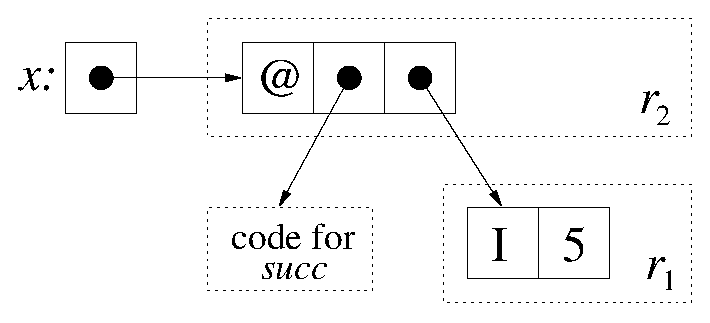
\includegraphics[scale=0.5]{2-System/fig/class-lazy}
\end{center}

\clearpage{}
\begin{center}
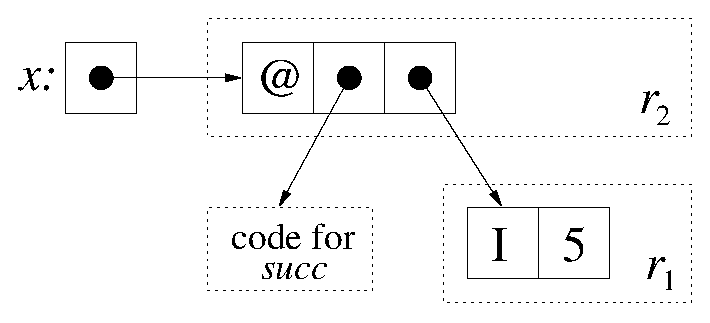
\includegraphics[scale=0.5]{2-System/fig/class-lazy}
\end{center}


As the application thunk represents a value of type $\iInt \ r_2'$ we draw it as belonging to the region $r_2$. This is opposed to thunks that represent partial applications. These thunks have no regions because they always represent objects of function type, and function types are not annotated with region variables.

When the value of $x$ is forced, the application $\isucc \ 5$ will be evaluated. Following lazy evaluation, the thunk will then be overwritten by an indirection node pointing to the result:

\begin{center}
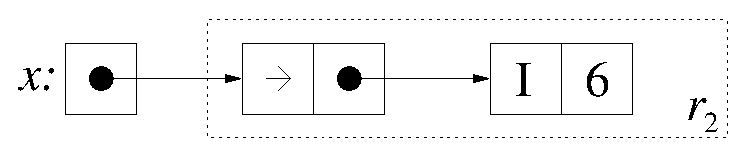
\includegraphics[scale=0.5]{2-System/fig/class-lazy-indir}
\end{center}

During back end code generation, we must account for the fact that $x$ may point to a thunk or indirection. To extract the unboxed integer from $x$ we must first load the tag of the object pointed to. This allows us to identify the sort of object it is, and decide whether to force the thunk, follow the indirection, or load the value as required. On the other hand, if we knew that $x$ was direct, as with:

\code{
	$x$	& $::$ 	& $\iInt \ r_2' \ \rhd \ \iDirect \ r_2'$ \\
}

Then we would be sure that $x$ only pointed to a boxed integer. This would save us from having to load the tag and do the test. Similarly to the way non-mutable regions default to being constant, non-lazy regions default to being direct.

\subsection{Liftedness is not a capability}
\label{System:Effects:liftedness}

We should note that the constraint names $\iLazy$ and $\iDirect$ have an operational flavour because DDC uses this information to guide optimisations. We could perhaps rename them to $\iLifted$ and $\iUnlifted$, which would reflect the fact that a $\iLifted$ value represents a computation that may diverge. 

A similar approach is taken in \cite{launchbury:unboxing-unpointed-types} and \cite{peyton-jones:bridging-the-gulf}, though they distinguish between pointed and lifted types. In \cite{launchbury:unboxing-unpointed-types}, the type of unlifted integers is written $\iInt^{\#}$. The type of lifted integers is defined to be $\iInt^{\#}_{\bot}$, with the $\bot$ in the subscript acting as a type operator that allows the bottom element to be one of the ``values'' represented by the type. Note that with this formulation, monotypes such as integers must be either lifted or unlifted. 

Our method of attaching constraints to region variables allows us to reuse the type class machinery to encode a similar property. However, type class constraints express a ``supports'' relationship, which doesn't quite match up with the concept of liftedness. For example, the constraint $\iEq \ a$ means that $a$ is a type whose values support being tested for equality. The constraint $\iMutable \ r$ means that the objects in region $r$ support being updated. Likewise, $\iConst \ r$ means that the objects in $r$ can be safely read by a suspended computation, that is, they support laziness. If an object is constrained to be neither $\iMutable$ nor $\iConst$ then we cannot assume it is safe to do either of these things. 

Extensionally, if a type is completely unconstrained then we know nothing about the values that inhabit that type. Each new constraint provides a new piece of information, and that information gives us the capability to do something new with the corresponding values.

If a region is $\iDirect$ then we can generate faster code to read objects in that region, because they are guaranteed not to be represented by thunks. However, the fact that a region is $\iLazy$ doesn't provide us with an additional capability. $\iLazy$ constraints are used only to ensure that a region is not also treated as $\iDirect$, as once we add thunks to a region we must test for them when reading every object from that region. In this sense, $\iLazy$ is a sort of ``anti-capability'' that indicates that a region has definitely been polluted by thunks and can no longer be used ``directly''.

For example, consider the following type:

\code{
	$\ifun :: \forall r_1 \ r_2. \ \iInt \ r_1 \to \iInt \ r_2$
}

As $r_1$ is unconstrained, objects passed to this function \emph{may} be represented by thunks. If instead we had:

\code{
	$\ifun :: \forall r_1 \ r_2. \ \iInt \ r_1 \to \iInt \ r_2 \ \rhd \ \iDirect \ r_1$
}

Then objects passed to the function are guaranteed \emph{not} to be represented by thunks, and we can optimise the function using this information. On the other hand, if we had:

\code{
	$\ifun :: \forall r_1 \ r_2. \ \iInt \ r_1 \to \iInt \ r_2 \ \rhd \ \iLazy \ r_1$
}

The $\iLazy$ constraint says that objects passed to this function may be represented by thunks, but this isn't new information compared with the first version. However, during type inference, if we discover that a term has type:

\code{
	$\iInt \ r_1 \rhd \iLazy \ r_1, \ \iDirect \ r_1$
}

Then this could mean that a lazy object, which might be a thunk, was passed to a function that can only accept a direct object, which cannot be a thunk. This is invalid, and will be marked as a type error.

